\documentclass[12pt,bibtotoc]{article}
\usepackage[table]{xcolor}
\usepackage[ngerman]{babel} % Für Silbentrennung
\usepackage[utf8]{inputenc} % Um Umlaute und Sonderzeichen nutzen zu können
\usepackage[a4paper,
lmargin={2cm},
rmargin={2cm},
tmargin={2cm},
bmargin={3cm}]{geometry} % Für das Layout
\usepackage{setspace} % Für den Zeilenabstand
\setstretch{1.25}
\usepackage{graphicx} % Um Bilder einzufügen
\usepackage{wrapfig} % Um Bilder im Fließtext einzubinden
\usepackage{csquotes} % Um Text in Anführungsstriche zu setzen
\usepackage{mathptmx} % Ähnlich zu Times New Roman
\usepackage{fancyhdr} % Um den Header einzufügen
\usepackage{pdfpages} % Um die Titelseite einbinden
\usepackage{hyperref} % Um Verlinkungen einfügen
\usepackage{acronym} % Um Akronyme zu definieren
\usepackage{textcomp} % Um spezielle Zeichen verwenden zu können (z.B. °, µ)
\usepackage{subcaption} % Um mehrere Bilder zusammen einzustellen und Links zu Abbildungen zu korrigieren


\usepackage[backend=bibtex, citestyle=ieee]{biblatex} % Um Literatur einzufügen
\bibliography{Quellenverzeichnis}

\pagestyle{fancy}
\fancyhf{}
\setlength\headheight{42.0pt}
\renewcommand{\headrulewidth}{0pt} % Um schwarze Linie zu entfernen
\chead{\includegraphics[width=\textwidth]{Resources/header.png}} % Grafik einfügen
\cfoot{\thepage}

\newcounter{romanBeginningEnd} % Um Römische Seitenzahl zu speichern

% Sektionen refernezen anpassen
\addto\extrasngerman{%
	\renewcommand{\sectionautorefname}{siehe}%
	\let\subsectionautorefname\sectionautorefname%
	\let\subsubsectionautorefname\sectionautorefname%
}



\begin{document}
    \pagenumbering{gobble}
    \newpage




\definecolor{color_30879}{rgb}{0,0.12549,0.376471}
\vspace{20mm}
\noindent
{\fontsize{15.96}{1}\usefont{T1}{cmr}{m}{n}\selectfont\color{color_30879}Transferleistung Theorie/Praxis  }\\ 
{\fontsize{15.96}{1}\usefont{T1}{cmr}{m}{n}\selectfont\color{color_30879}Nr. X} 

\vspace{15mm}



\begin{center}
\begin{tabular}{ |>{\columncolor{color_30879}}p{1.6in} | p{4.4in}| } 
 \hline
 \textcolor{white}{Martrikelnummer:} & Martrikelnummer \\[0.2in]
 \hline
 \textcolor{white}{Freigegebenes Thema:} & Thema \\ [1in]
 \hline
 \textcolor{white}{Studiengang, Zenturie:} & Studiengang/Zenturie \\ [0.2in]
 \hline
\end{tabular}
\end{center}

	%\includepdf[pages=-]{Resources/cover}
	
	\setcounter{page}{1} % Römische Seitenzahlen
	\pagenumbering{Roman}
	
	\tableofcontents %Inhaltsverzeichnis
	\newpage
	
	\setcounter{secnumdepth}{0} % Keine Numerierung von Überschriften
	\clearpage
	\phantomsection
	\addcontentsline{toc}{section}{\listfigurename} % Abbildungsverzeichnis im Inhaltsverzeichnis anzeigen
	\listoffigures
	\clearpage
	\phantomsection
	\addcontentsline{toc}{section}{\listtablename} % Abbildungsverzeichnis im Inhaltsverzeichnis anzeigen
	\listoftables
	\newpage
	\section{Abkürzungsverzeichnis}
	% Abkürzungen
	\begin{acronym}[LängsteAbkürzung] % Für Formatierung längste Abkürzung eintragen
		\acro{ac:Label}[Abkürzung]{LangForm}
	\end{acronym}
	\newpage
	
	\setcounter{secnumdepth}{3} % Überschriften wieder numerieren
	
	\setcounter{romanBeginningEnd}{\the\value{page}} % Speichern der römischen Seitenzahl
	\setcounter{page}{1} % Mit Arabischen Seitenzahlen wieder bei 1 anfangen
	\pagenumbering{arabic}
	
	% ###############################################################
	% Hier Inhalt einfügen
	\section{Beispielsection}
Lorem Ipsum\cite{ref:cis} dolor sit amet, consetetur sadipscing elitr, sed diam nonumy eirmod tempor invidunt ut labore et dolore magna aliquyam erat, sed diam voluptua. At vero eos et accusam et justo duo dolores et ea rebum. Stet clita kasd gubergren, no sea takimata sanctus est Lorem ipsum dolor sit amet. Lorem ipsum dolor sit amet, consetetur sadipscing elitr, sed diam nonumy eirmod tempor invidunt ut labore et dolore magna aliquyam erat, sed diam voluptua. At vero eos et accusam et justo duo dolores et ea rebum. Stet clita kasd gubergren, no sea takimata sanctus est Lorem ipsum dolor sit amet.

\begin{figure} [h!]
\centering
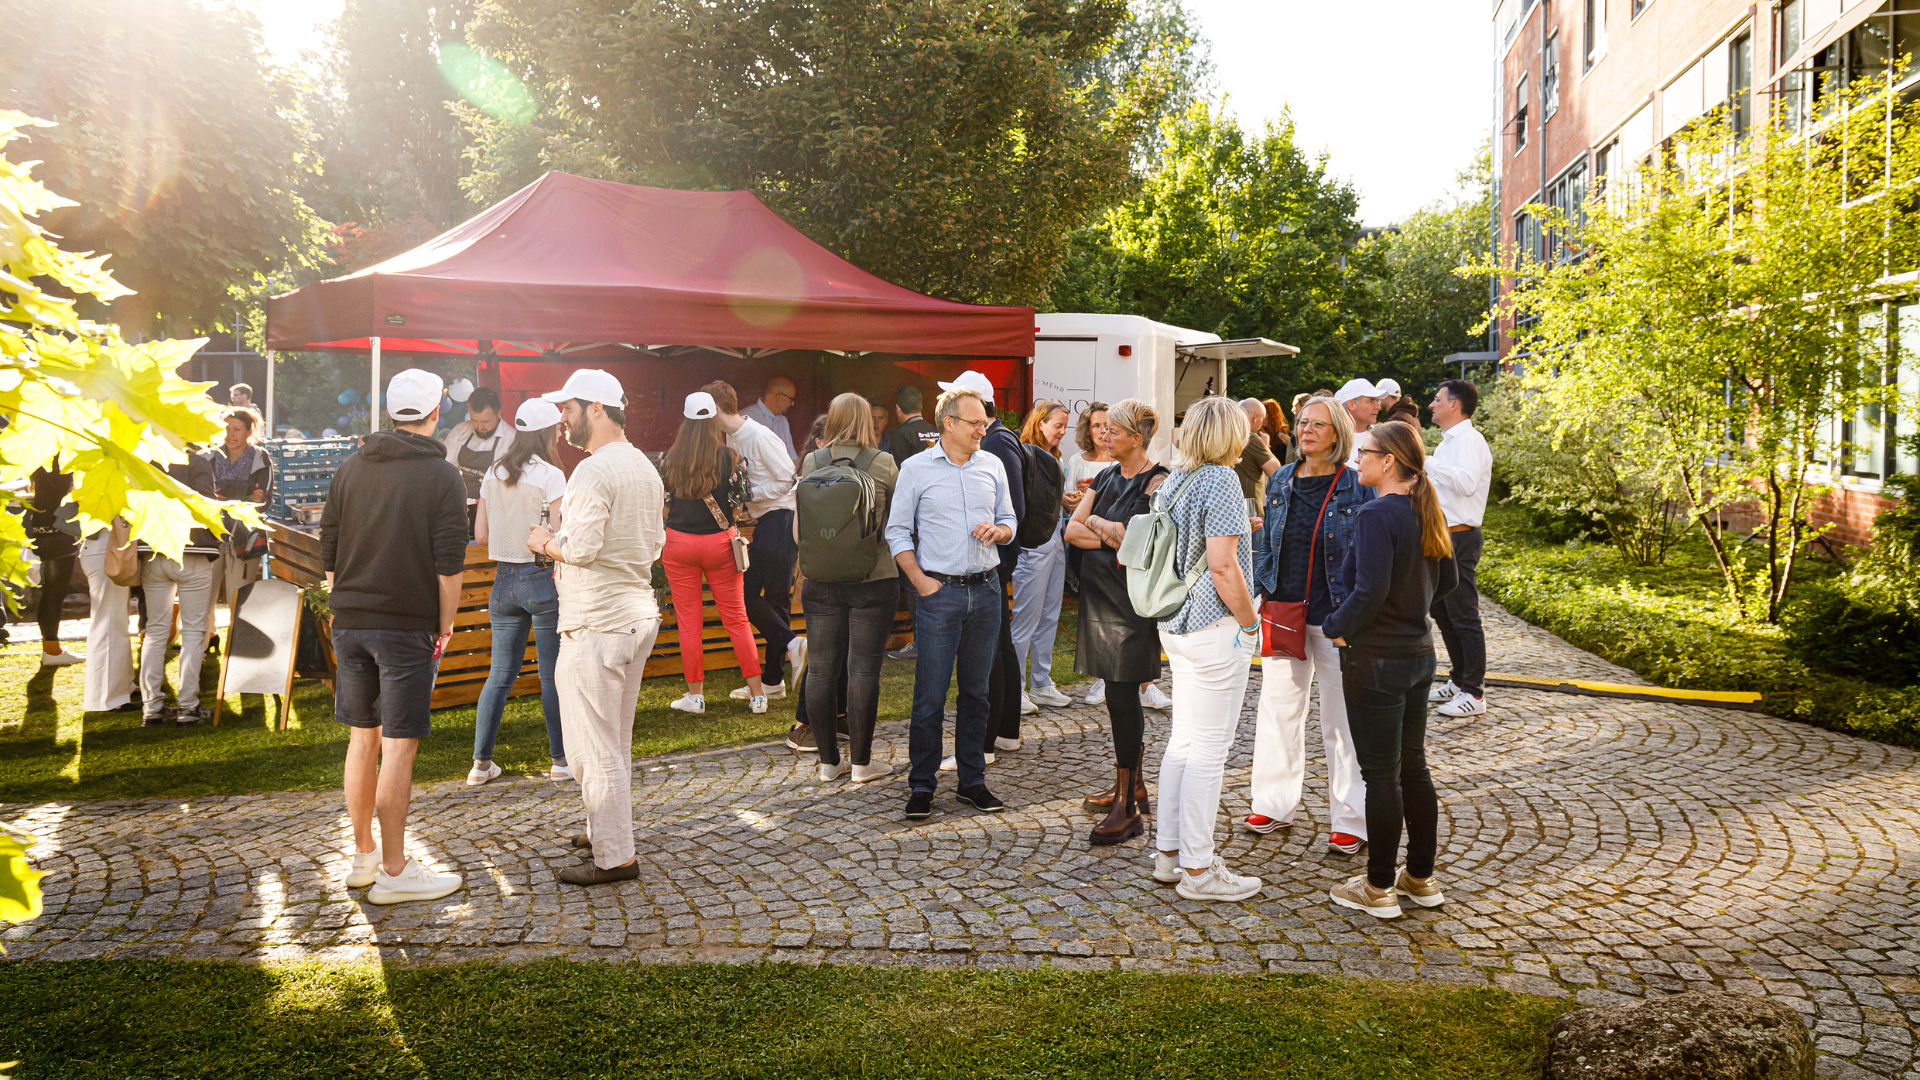
\includegraphics[scale=0.1]{Resources/Hochschulleben.png}
\caption{Hochschulleben}
\label{fig:figure3}
\end{figure}

\subsection{Untersektion}
At vero eos et accusam et justo duo dolores et ea rebum. Stet clita kasd gubergren, no sea takimata \cite{Book:1} sanctus est Lorem ipsum dolor sit amet. Lorem ipsum dolor sit amet, consetetur sadipscing elitr, sed diam nonumy eirmod tempor invidunt ut labore et dolore magna aliquyam erat, sed diam voluptua. At vero eos et accusam et justo duo dolores et ea rebum. Stet clita kasd gubergren, no sea takimata sanctus est Lorem ipsum dolor sit amet.   

Duis autem vel eum iriure dolor in hendrerit in vulputate velit esse molestie consequat, vel illum dolore eu feugiat nulla facilisis at vero eros et accumsan et iusto odio dignissim qui blandit praesent luptatum zzril delenit augue duis dolore te feugait nulla facilisi. Lorem ipsum dolor sit amet,


\begin{table}[h]
\centering
 \begin{tabular}{||c c c c||} 
 \hline
 Col1 & Col2 & Col2 & Col3 \\ [0.5ex] 
 \hline\hline
 1 & 6 & 87837 & 787 \\ 
 \hline
 2 & 7 & 78 & 5415 \\
 \hline
 3 & 545 & 778 & 7507 \\
 \hline
 4 & 545 & 18744 & 7560 \\
 \hline
 5 & 88 & 788 & 6344 \\ [1ex] 
 \hline
 \end{tabular}
\caption{Interessante Daten}
\label{tab:table1}
\end{table}

	% ###############################################################
	
	\newpage
	\pagenumbering{Roman}
	\setcounter{page}{\theromanBeginningEnd} % Römische Seitenzahlen fortsetzen
	\setcounter{secnumdepth}{0} % Nummerierung der Überschriften entfernt
	\section{Quellenverzeichnis}
	\setcounter{secnumdepth}{3} % Überschriften wieder numerieren (Für den Anhang)
	\printbibliography[heading=none]
	\newpage
	\appendix
\section{Dies ist ein TestAnhang}

\end{document}